%%%%%%%%%%%%%%%%%%%%%%%%%%%%%%%%%%%%%%%%%%%%%%%%%%%%%%%%%%%%%%%%%%%%%%%%%%%%%%%%
% app_glossary.tex: Glossary Appendix:
%%%%%%%%%%%%%%%%%%%%%%%%%%%%%%%%%%%%%%%%%%%%%%%%%%%%%%%%%%%%%%%%%%%%%%%%%%%%%%%%
\chapter{Electron Results}
\label{app_glossary}
%%%%%%%%%%%%%%%%%%%%%%%%%%%%%%%%%%%%%%%%%%%%%%%%%%%%%%%%%%%%%%%%%%%%%%%%%%%%%%%%
%%%%%%%%%%%%%%%%%%%%%%%%%%%%%%%%%%%%%%%%%%%%%%%%%%%%%%%%%%%%%%%%%%%%%%%%%%%%%%%%
The results of the \phistar measurement using only \xxbar{e}{e} data are shown in the following plots. The \xxbar{e}{e} is the sample that was combined with the \xxbar{\mu}{\mu} for the results shown in Sec. \ref{Sec:Blue}. Both the normalized and absolute 1D results are shown in Fig. \ref{fig:Unfoldedee1DResults}, while the 2D results are all normalized. 

%%%%%%%%%%%%%%%%%%%%%%%%%%%%%%%%%%%%%%%%%%%%%%%%%%%%%%%%%%%%%%%%%%%%%%%%%%%%%%%%
% Glossary {{{
%%%%%%%%%%%%%%%%%%%%%%%%%%%%%%%%%%%%%%%%%%%%%%%%%%%%%%%%%%%%%%%%%%%%%%%%%%%%%%%%
\label{jargonapp}
%%%%%%%%%%%%%%%%%%%%%%%%%%%%%%%%%%%%%%%%%%%%%%%%%%%%%%%%%%%%%%%%%%%%%%%%%%%%%%%%
\begin{figure}
    \centering
   \begin{subfigure}[b]{0.49\textwidth}
    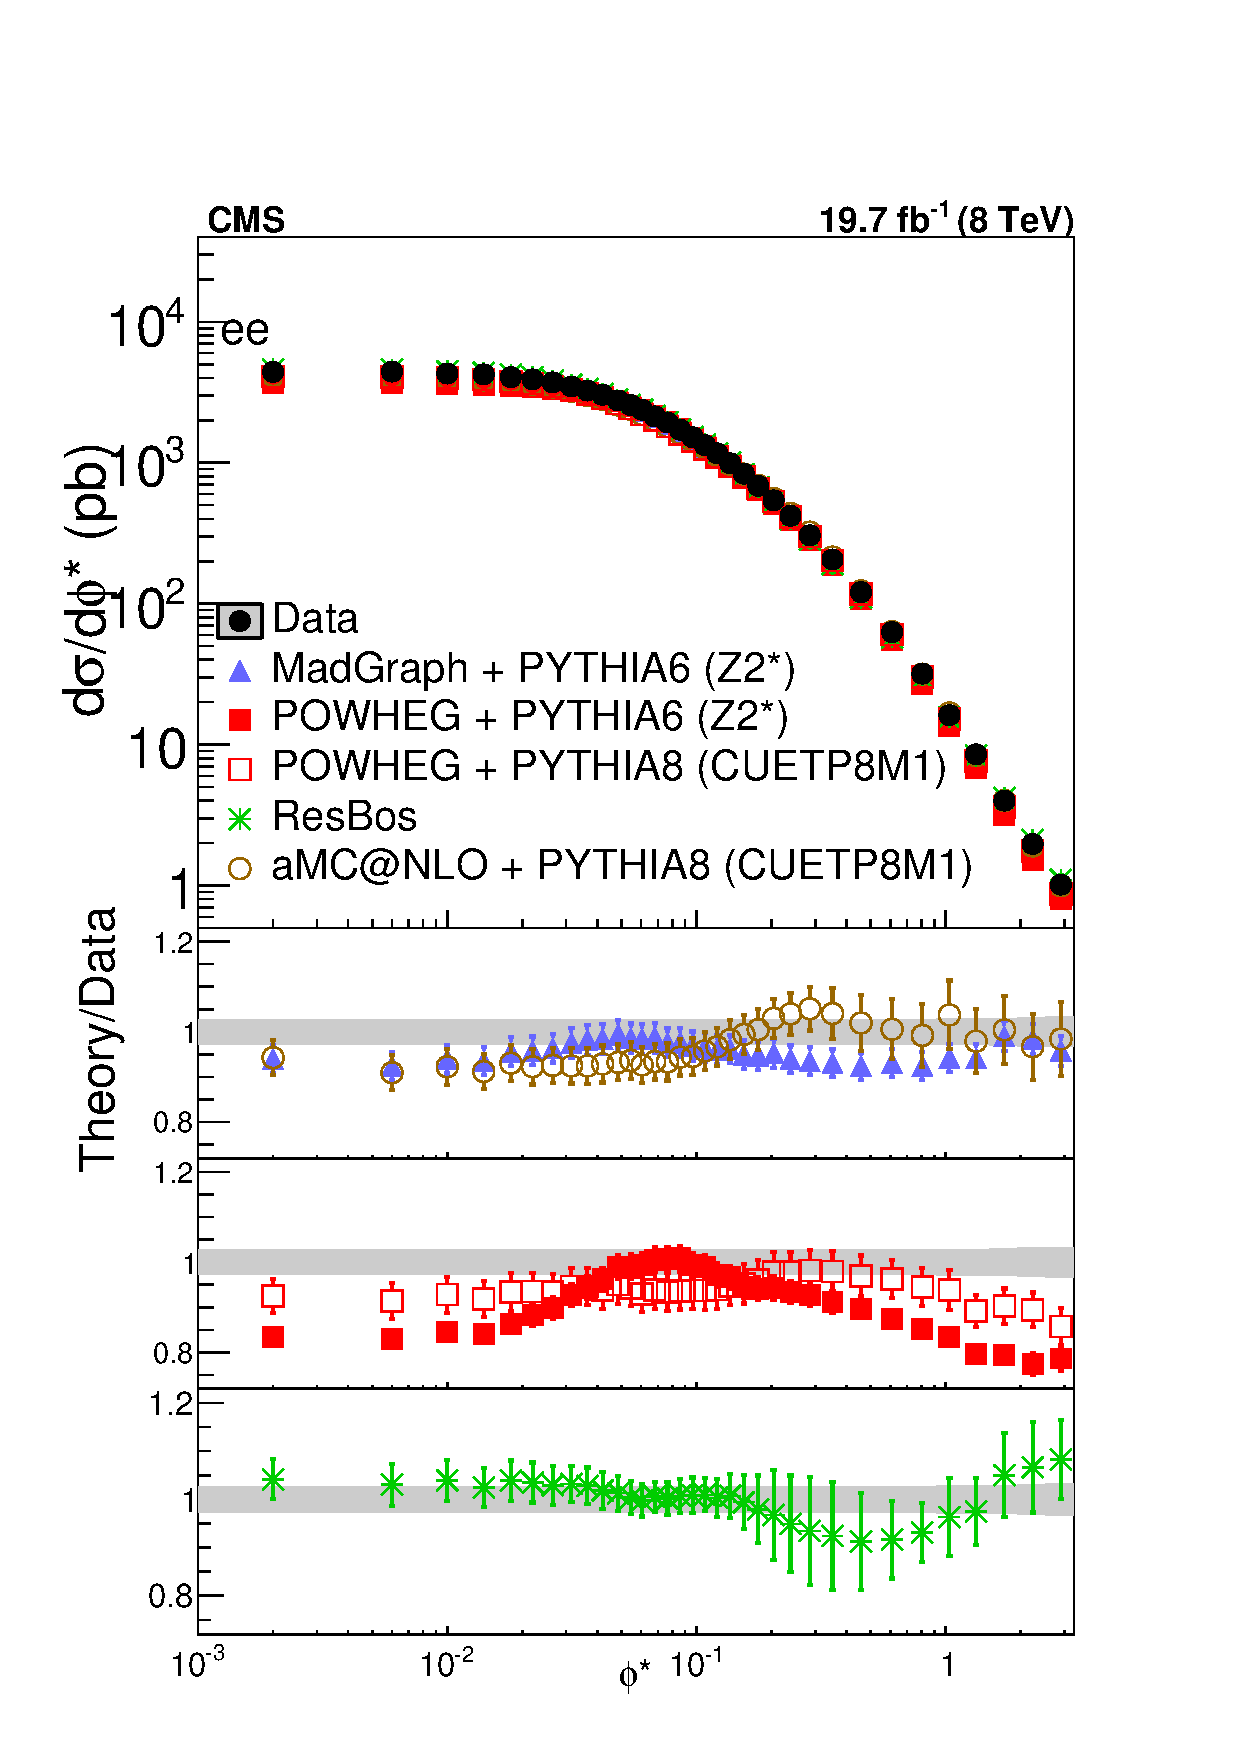
\includegraphics[width=\linewidth]{figures/AppendexA/ZShape_MGAndAMC_PowHegs_elec_Abs_Born.pdf}
    \end{subfigure}
    \begin{subfigure}[b]{0.49\textwidth}
    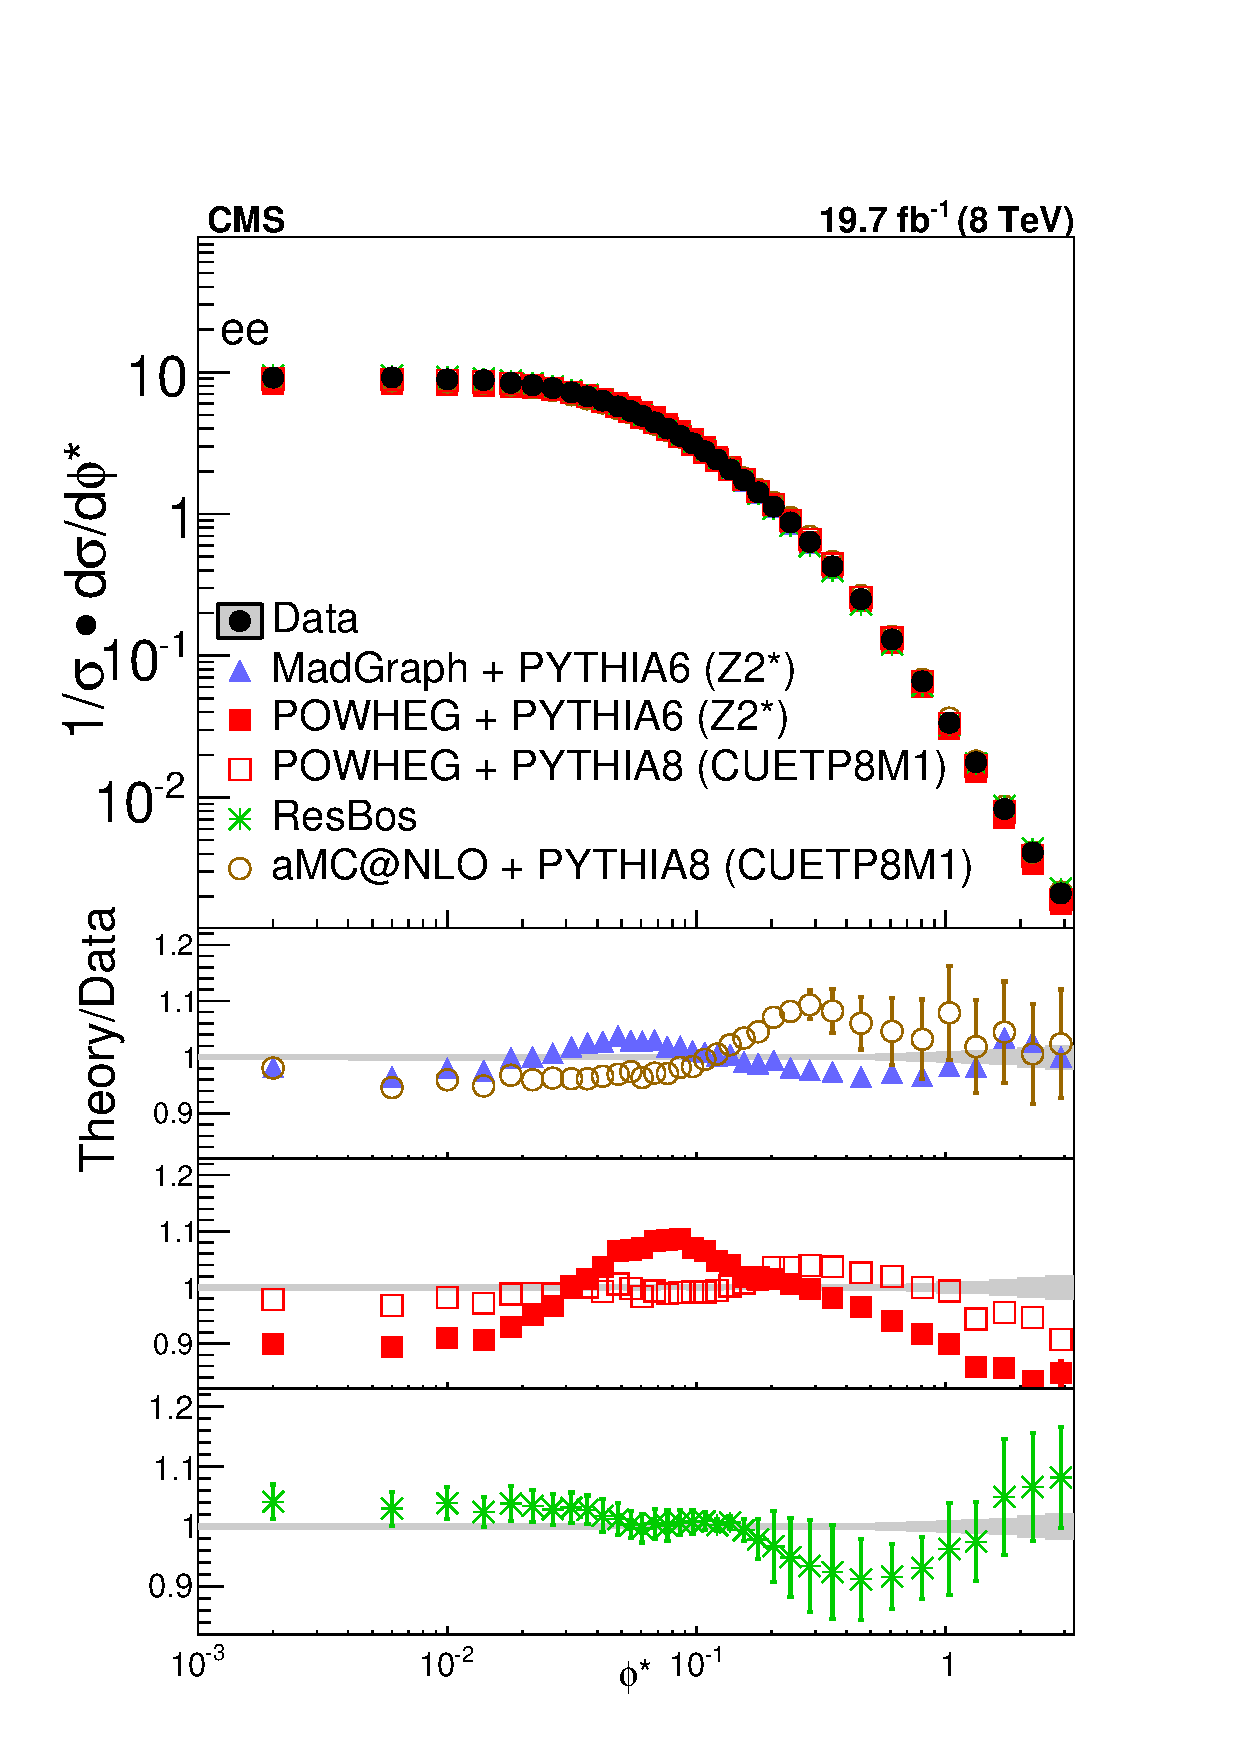
\includegraphics[width=\linewidth]{figures/AppendexA/ZShape_MGAndAMC_PowHegs_elec_Norm_Born.pdf}
    \end{subfigure}
    \caption[\xxbar{e}{e} 1D results]{\xxbar{e}{e} 1D results. The left figure shows the absolute \phistar distribution compared to five separate simulation samples while the right compares the same distributions after they have been normalized.}
    \label{fig:Unfoldedee1DResults}
\end{figure}



\begin{figure}
    \centering
    \hspace*{-2cm}
    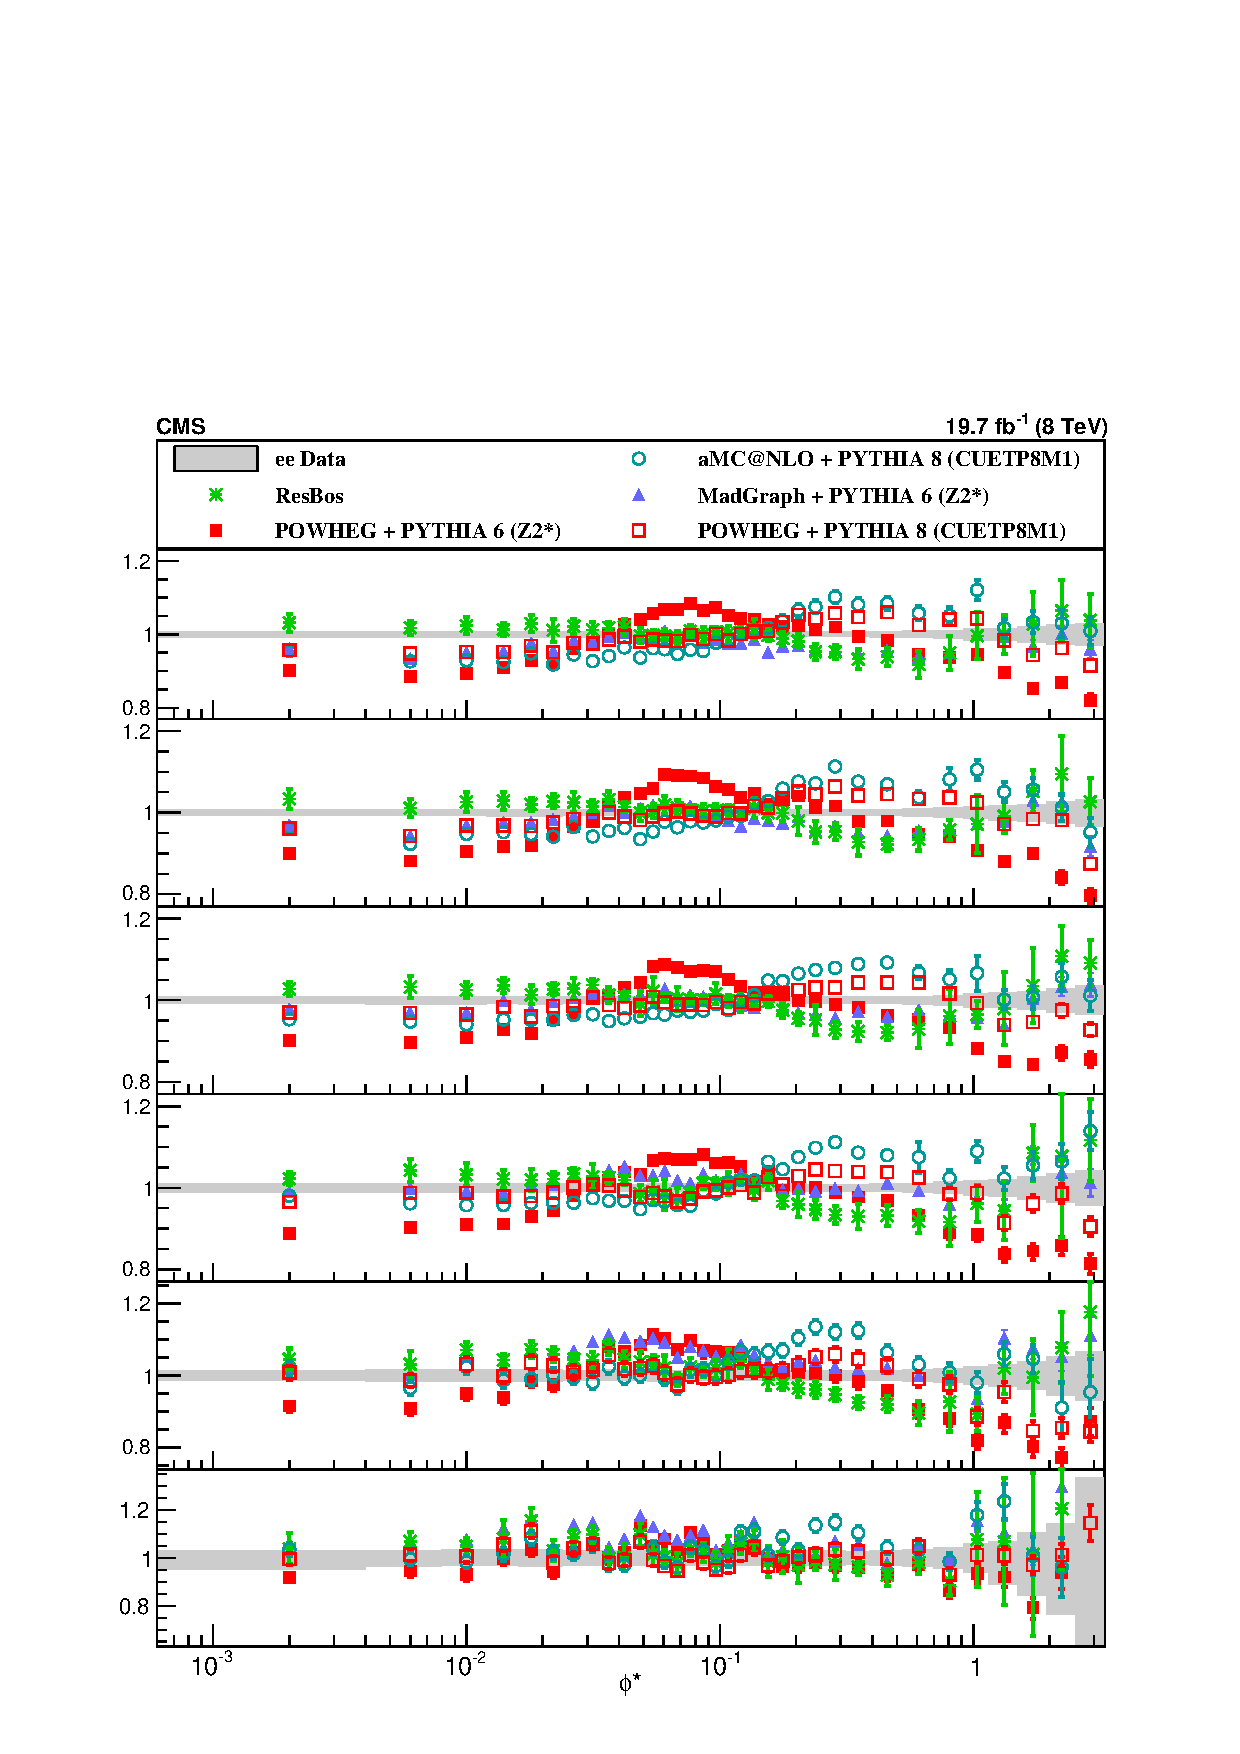
\includegraphics{figures/AppendexA/Ratio_ZShape_2D_ALLelec_PH_Norm_Born.pdf}
    \caption[\xxbar{e}{e} 2D results]{Normalized \xxbar{e}{e} 2D results.}
    \label{fig:2DElectrons}
\end{figure}{}

\begin{figure}
    \centering
    \hspace*{-2cm}
    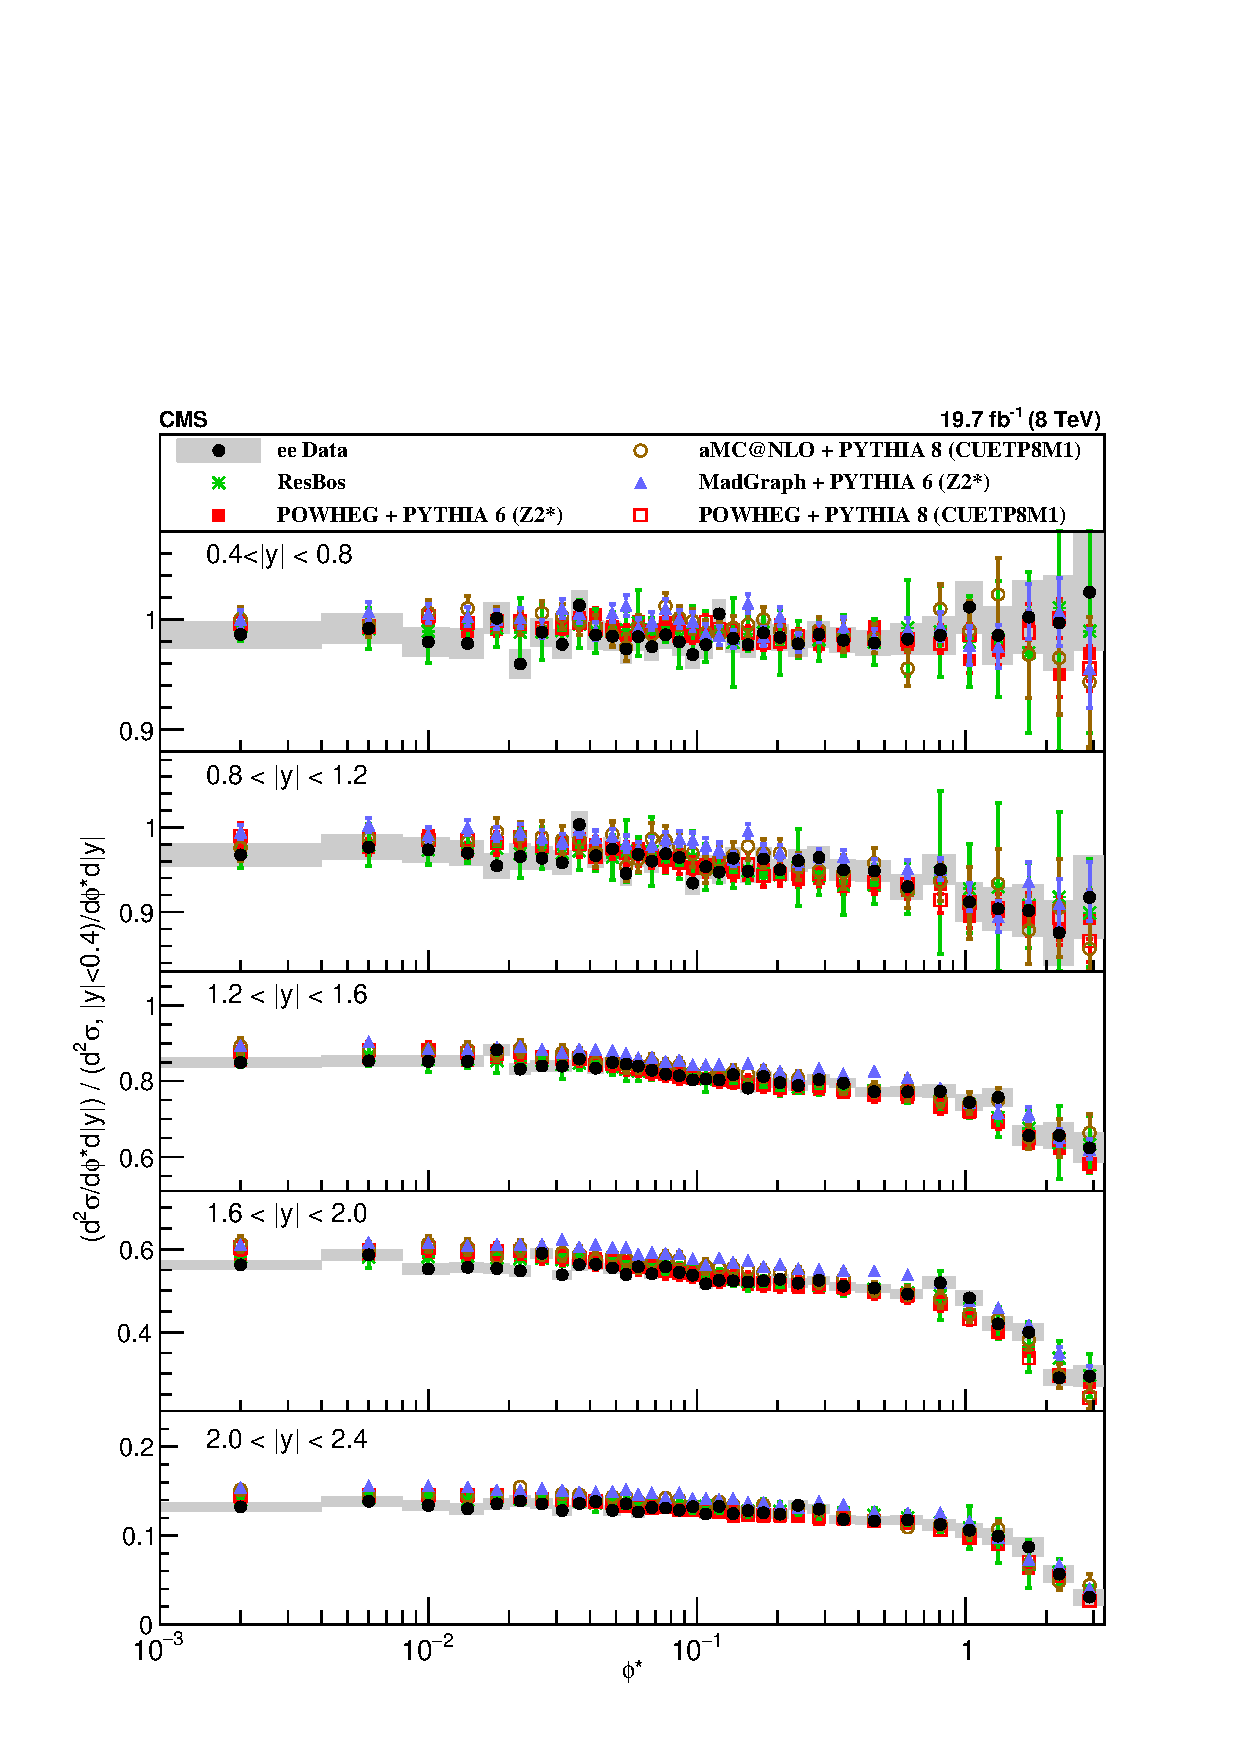
\includegraphics{figures/AppendexA/PowHegBin0RatElectron.pdf}
    \caption[\xxbar{e}{e} rapidity bins compared with bin0]{This shows the ratio of all other \phistar distributions at all rapidity regions to the region $|\rapidity|<0.4$}
    \label{fig:my_label}
\end{figure}
%%%%%%%%%%%%%%%%%%%%%%%%%%%%%%%%%%%%%%%%%%%%%%%%%%%%%%%%%%%%%%%%%%%%%%%%%%%%%}}}
